\pdfminorversion=6
\documentclass[letterpaper]{article}
\usepackage[preprint]{aaai2027}
\usepackage[hyphens]{url}
\usepackage{graphicx}
\urlstyle{rm}
\def\UrlFont{\rm}
\usepackage{natbib}
\usepackage{caption}
\usepackage{booktabs}
\usepackage{amsmath}
\usepackage{amssymb}
\usepackage{tikz}
\definecolor{IdeaBlue}{HTML}{274C77}
\definecolor{ImplCoral}{HTML}{E76F51}
\definecolor{EvalTeal}{HTML}{2A9D8F}
\definecolor{AuditGold}{HTML}{A66B00}
\definecolor{SoftGray}{HTML}{EEF2F4}
\frenchspacing

\pdfinfo{
/TemplateVersion (2027.1)
}

\setcounter{secnumdepth}{1}

\title{One Run Is Not an Idea: The Implementation Lottery in Automated Research}
\author{Jingjie Ning, Shanshan Zhong, Xiaochuan Li, Ji Zeng, Chenyan Xiong}
\affiliations{
School of Computer Science, Carnegie Mellon University\\
\{jening,szhong2,xiaochu4,jizeng,cx\}@cs.cmu.edu
}

\begin{document}

\maketitle

\begin{abstract}
Automated research systems use experimental scores both to deliver artifacts and to decide which ideas to retain, transfer, and pursue. Yet one run scores one implementation of an idea. Crediting that realization-level score as evidence about the parent mechanism creates the \emph{implementation lottery}, in which an idea-level conclusion depends on which plausible implementation was sampled. The mismatch is structural whenever one run updates beliefs about a mechanism. We estimate its magnitude. The \emph{Idea Reliability Audit} measures \emph{idea reliability} by validating and freezing candidate cards, sampling fresh-session implementations, using outcome-blind fidelity labels, and rerunning saved artifacts. It reports idea ICC and leave-one-implementation-out (LOO) winner reversal. Prior work generally repeats the task; we repeat the idea. Across 312 assignments on 13 tabular tasks and two coding-agent setups, implementation variance was more than five and ten times same-artifact rerun variance, respectively, and the winner from one implementation draw differed from the winner under the other-two mean in 25.6\% and 43.6\% of decisions. Reversal survives card-level filtering under two outcome-blind review rules. An exploratory diagnostic on three materials-regression workflows with a deterministic evaluator also finds implementation variation dominating the decomposition. These findings distinguish idea reliability from best-of-$N$ artifact utility. Before a score guides idea-level branching, transfer, or research memory, evidence should cover multiple implementations.
\end{abstract}

\section{Introduction}

We use \emph{automated research} to describe a closed loop that proposes, implements, tests, and selects research directions. The AI Scientist, Dolphin, and Agent Laboratory automate growing parts of this loop \cite{lu2024aiscientist,yuan2025dolphin,schmidgall2025agentlab}. Tree-search variants explicitly explore candidate artifacts \cite{yamada2025aiscientistv2}, while executable benchmarks ask agents to improve concrete programs \cite{nathani2025mlgym,garikaparthi2026researchgym}. Exploring several realizations and retaining the best is appropriate when the deliverable is that artifact.

The same loop also uses results to decide what research to pursue. Scientific learning then asks whether a selected result is evidence for the named idea, so it can guide branching, transfer, and cumulative knowledge. A selected maximum identifies what one search budget found. It need not rank ideas as they perform across plausible implementations. This distinction matters when systems use their own experiments to allocate future research effort \cite{wang2023scientificdiscovery}.

Suppose an agent proposes early stopping for a booster. The mechanism fixes a training-only validation set, a stopping rule, and restoration of the best iteration. Faithful implementations may still choose the validation fraction, patience, monitored metric, and library interface. The score from one run therefore measures both the fixed idea and one realization of its permitted choices. An illustrative case from our audits makes the consequence concrete. Three valid, blind-faithful implementations of one frozen card span $+2.31\%$ to $-1.85\%$, while all same-artifact reruns are exact. Against the same competitor, every one-draw winner reverses under the other-two mean (Figure~\ref{fig:case}).

Trying several realizations and keeping the maximum can improve the returned artifact, but it does not resolve attribution. The maximum targets an upper tail and can favor ideas with greater implementation variance or search effort. That is useful for delivery but consequential when the score is credited to the idea and steers the next hypothesis.

\begin{figure*}[t]
\centering
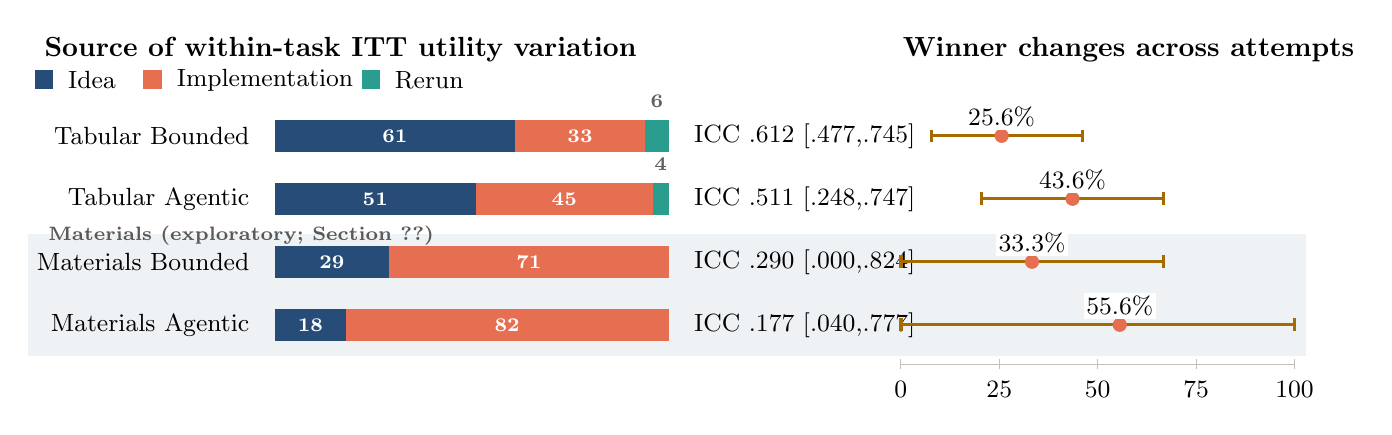
\begin{tikzpicture}[font=\small]
\fill[SoftGray] (-0.08,0.55) rectangle (16.15,2.10);
\node[anchor=west,font=\bfseries] at (0,4.45) {Source of within-task ITT utility variation};
\node[anchor=west,font=\bfseries] at (10.9,4.45) {Winner changes across attempts};
\fill[IdeaBlue] (0,3.95) rectangle +(0.23,0.23);
\node[anchor=west] at (0.30,4.06) {Idea};
\fill[ImplCoral] (1.38,3.95) rectangle +(0.23,0.23);
\node[anchor=west] at (1.68,4.06) {Implementation};
\fill[EvalTeal] (4.15,3.95) rectangle +(0.23,0.23);
\node[anchor=west] at (4.45,4.06) {Rerun};
\node[anchor=east] at (2.85,3.35) {Tabular Bounded};
\fill[IdeaBlue] (3.05,3.15) rectangle (6.10,3.55);
\fill[ImplCoral] (6.10,3.15) rectangle (7.75,3.55);
\fill[EvalTeal] (7.75,3.15) rectangle (8.05,3.55);
\node[text=white,font=\scriptsize\bfseries] at (4.575,3.35) {61};
\node[text=white,font=\scriptsize\bfseries] at (6.925,3.35) {33};
\node[anchor=south,text=gray!75!black,font=\scriptsize\bfseries] at (7.90,3.58) {6};
\node[anchor=west] at (8.25,3.35) {ICC .612 [.477,.745]};
\node[anchor=east] at (2.85,2.55) {Tabular Agentic};
\fill[IdeaBlue] (3.05,2.35) rectangle (5.60,2.75);
\fill[ImplCoral] (5.60,2.35) rectangle (7.85,2.75);
\fill[EvalTeal] (7.85,2.35) rectangle (8.05,2.75);
\node[text=white,font=\scriptsize\bfseries] at (4.325,2.55) {51};
\node[text=white,font=\scriptsize\bfseries] at (6.725,2.55) {45};
\node[anchor=south,text=gray!75!black,font=\scriptsize\bfseries] at (7.95,2.78) {4};
\node[anchor=west] at (8.25,2.55) {ICC .511 [.248,.747]};
\node[anchor=west,font=\scriptsize\bfseries,text=gray!70!black] at (0.05,2.08)
      {Materials (exploratory; Section~\ref{sec:materials})};
\node[anchor=east] at (2.85,1.75) {Materials Bounded};
\fill[IdeaBlue] (3.05,1.55) rectangle (4.50,1.95);
\fill[ImplCoral] (4.50,1.55) rectangle (8.05,1.95);
\node[text=white,font=\scriptsize\bfseries] at (3.775,1.75) {29};
\node[text=white,font=\scriptsize\bfseries] at (6.275,1.75) {71};
\node[anchor=west] at (8.25,1.75) {ICC .290 [.000,.824]};
\node[anchor=east] at (2.85,0.95) {Materials Agentic};
\fill[IdeaBlue] (3.05,0.75) rectangle (3.95,1.15);
\fill[ImplCoral] (3.95,0.75) rectangle (8.05,1.15);
\node[text=white,font=\scriptsize\bfseries] at (3.50,0.95) {18};
\node[text=white,font=\scriptsize\bfseries] at (6.00,0.95) {82};
\node[anchor=west] at (8.25,0.95) {ICC .177 [.040,.777]};
\draw[gray!50] (11.0,0.45) -- (16.0,0.45);
\foreach \x/\lab in {11.0/0,12.25/25,13.5/50,14.75/75,16.0/100} {\draw[gray!50] (\x,0.39)--(\x,0.51); \node[anchor=north] at (\x,0.35) {\lab};}
\draw[AuditGold,line width=1.2pt] (11.385,3.35)--(13.31,3.35);
\draw[AuditGold,line width=1.2pt] (11.385,3.27)--(11.385,3.43) (13.31,3.27)--(13.31,3.43);
\fill[ImplCoral] (12.28,3.35) circle (0.09);
\node[anchor=south,fill=white,inner sep=1pt] at (12.28,3.42) {25.6\%};
\draw[AuditGold,line width=1.2pt] (12.025,2.55)--(14.335,2.55);
\draw[AuditGold,line width=1.2pt] (12.025,2.47)--(12.025,2.63) (14.335,2.47)--(14.335,2.63);
\fill[ImplCoral] (13.18,2.55) circle (0.09);
\node[anchor=south,fill=white,inner sep=1pt] at (13.18,2.62) {43.6\%};
\draw[AuditGold,line width=1.2pt] (11.0,1.75)--(14.335,1.75);
\draw[AuditGold,line width=1.2pt] (11.0,1.67)--(11.0,1.83) (14.335,1.67)--(14.335,1.83);
\fill[ImplCoral] (12.665,1.75) circle (0.09);
\node[anchor=south,fill=white,inner sep=1pt] at (12.665,1.82) {33.3\%};
\draw[AuditGold,line width=1.2pt] (11.0,0.95)--(16.0,0.95);
\draw[AuditGold,line width=1.2pt] (11.0,0.87)--(11.0,1.03) (16.0,0.87)--(16.0,1.03);
\fill[ImplCoral] (13.78,0.95) circle (0.09);
\node[anchor=south,fill=white,inner sep=1pt] at (13.78,1.02) {55.6\%};
\end{tikzpicture}
\caption{The implementation lottery in the primary Tabular audit (top) under capped-call Bounded and SDK-session Agentic setups, and in the exploratory Materials diagnostic (shaded). Stacked bars show the share of within-task intention-to-treat (ITT) variance due to frozen candidate, implementation, and same-artifact rerun. The idea ICC equals the first share. Points show LOO reversal with 95\% task-level intervals. Tabular uses all frozen candidates. Card-filtered sensitivities appear in Table~\ref{tab:portfolio-sensitivity}. Materials is never pooled with Tabular, and its rerun variance is zero because the evaluator is deterministic.}
\label{fig:main}
\end{figure*}

Written ideas can be rated for novelty and feasibility \cite{si2025ideas}, and execution can change those ratings \cite{si2026gap}. One idea can admit several plausible implementations. We call dependence on one sampled realization the \textbf{implementation lottery}. \textbf{Idea reliability} is the stability of idea-level evidence across implementations; the \textbf{Idea Reliability Audit} estimates it. Prior repeated-run evaluations treat a task or query as the repeated object. We instead hold a mechanism-level idea fixed, repeat its translation into artifacts, audit semantic adherence, and separately rerun saved artifacts.

Automated research often makes idea-level decisions from one realization. This unit mismatch is structural; only its magnitude is empirical. Our audits find 25.6--43.6\% selection reversal (Figure~\ref{fig:main}). We make three contributions.

\begin{itemize}
\item \textbf{Phenomenon and scale.} Across 312 assignments on 13 tabular tasks, implementation variance exceeds same-artifact rerun variance by more than fivefold for Bounded and tenfold for Agentic. LOO winner reversal occurs in 25.6\% and 43.6\% of decisions.
\item \textbf{Measurement target.} We formalize idea reliability as the stability of evidence across independent idea-to-artifact runs. We distinguish average-realization operational idea quality $Q$ from best-of-$N$ artifact utility $B_N$ and connect ICC to winner stability.
\item \textbf{Instrument.} We introduce an audit that checks portfolio validity, freezes cards, samples fresh-session implementations, labels fidelity, and reruns identical artifacts. It reports idea ICC, LOO reversal, and task-level uncertainty.
\end{itemize}

To our knowledge, this is the first study to hold a research idea semantically fixed while repeatedly sampling its translation into artifacts. This design separates implementation variance from same-artifact rerun noise and uses outcome-blind fidelity review. It is also the first to report idea-level selection reversal caused by resampling independent implementations of a fixed idea portfolio. The results compare implementation variation with rerun noise, examine both processes and a fully valid case, repeat the analysis after outcome-blind card filtering, and provide an exploratory Materials check. In a closed loop, a realization-specific winner can redirect later experiments. Search determines what to deploy; idea reliability determines what the research loop should remember.

\section{Idea Reliability as Measurement}

\subsection{What One Score Contains}

A task context fixes data, code, split, metric, and compute budget. An idea states a mechanism while leaving reasonable implementation choices open. An agent turns it into code, which an evaluator scores. Repetition separates variation across ideas, across implementations of one idea, and across reruns of one saved implementation.

Let $s$ denote a task, $i$ an idea, $e$ a coding-agent setup, $j$ an independent implementation attempt, and $k$ a training or evaluation rerun. For a fixed setup $e$, we write the observed utility as
\begin{equation}
Y_{siejk} = \mu_e + A_{se} + I_{sie} + M_{siej} + R_{siejk},
\label{eq:nested}
\end{equation}
where $A$ is the task contribution, $I$ is the idea contribution within a task, $M$ is the implementation contribution within an idea, and $R$ is variation observed when the same implementation is rerun. The random terms are zero mean and exchangeable within each level. For a fixed task and implementation agent, operational idea quality is the average ITT utility over independent implementation attempts and evaluator reruns.
\begin{equation}
Q(s,i,e) = \mathbb{E}_{j,k}[Y_{siejk}].
\end{equation}
For decision quantities, let $Z_{siej}$ denote the implementation-level score exposed to the selector. In our experiments this is the frozen primary ITT utility, while separate same-artifact reruns estimate $\sigma_R^2$. Best-of-$N$ artifact search targets an upper-tail quantity such as $B_N(s,i,e)=\mathbb{E}[\max_{j\leq N}Z_{siej}]$. Both are legitimate estimands but answer different questions. $B_N$ describes what a budgeted search can return, whereas $Q$ describes the idea across realizations. Crediting a realization-level $Z$ as evidence about $Q$ creates the implementation lottery because the idea-level conclusion then depends on which plausible implementation was sampled. A change in the selected idea across implementation draws is its decision-level manifestation. This definition follows reliability and generalizability theory \cite{shrout1979icc,brennan2001generalizability}. The measured object is a research idea and the repeated measurements are its implementations.

\subsection{Two Measures of Reliability}

For each coding-agent setup, we estimate the variance components with a balanced nested analysis of variance. Negative sampling estimates are set to zero. Task variance is excluded because an automated research system compares ideas within the same task. The idea ICC is
\begin{equation}
\mathrm{ICC}_{\mathrm{idea}} =
\frac{\sigma_I^2}
{\sigma_I^2 + \sigma_M^2 + \sigma_R^2}.
\label{eq:icc}
\end{equation}
The ICC is the share of within-task ITT utility variation that separates ideas. A value near one means that independent implementation attempts preserve the idea signal. Lower values mean that one run is less representative.

The second measure asks whether implementation choice changes the winner. We form three one-draw worlds, each containing one implementation per idea, and ask whether each winner survives the other two implementations. The preregistered alignment $h\in\{1,2,3\}$ groups same-index draws across ideas into worlds; it is a label, not shared provider randomness. For each $h$, one draw selects
\begin{equation}
\hat{i}_{s,e,h} = \arg\max_i Z_{sieh},
\end{equation}
and we compare it with $\arg\max_i \bar{Z}_{sie,-h}$. This other-two mean is a finite-budget reference, not ground truth, so LOO measures decision stability rather than latent-ranking error. A disagreement is a leave-one-implementation-out (LOO) winner reversal. Exact observed ties select the lexicographically largest frozen idea label; reference means tied within $10^{-12}$ all count as best. Each task contributes three dependent decisions, so uncertainty is clustered by task.

These measures apply when a result prunes an idea branch, motivates transfer, enters research memory, or supports a mechanism-level claim. An audit draw may itself be a complete tree-search run; Section~\ref{sec:implications} discusses promotion policies.

\section{The Idea Reliability Audit}

Figure~\ref{fig:teaser} summarizes the prospective workflow. Each component addresses a distinct alternative explanation for an unstable idea-level decision.

\subsection{Mechanism-Level Idea Cards}

Mechanism-level cards rule out the alternative that variation reflects an underspecified slogan or a fully specified recipe. A card fixes the scientific intervention while leaving ordinary choices about models, features, preprocessing, and parameters open. It records the mechanism, required properties, open choices, expected result, and counterevidence. Exact constructors, hyperparameters, random seeds, and line-by-line steps are excluded because they define a recipe. Idea reliability is defined at this card granularity. Under our no-search policy, each draw is one translation; with tuning, the search procedure and budget become part of the implementation process being audited.

For example, one frozen tabular card fixes early stopping. It reserves training data for validation, monitors it during boosting, stops under a patience rule, and returns the best iteration under a 300-iteration ceiling. The executor still chooses the validation fraction, patience, metric, split seed, and built-in versus manual interface. Leaf regularization or feature subsampling would change the mechanism and violate the card.

For every task, cards are generated before implementation and remain blind to hidden outcomes. Frozen baseline development lineage remains visible. The task context fixes the data, code snapshot, split, metric, environment, and compute policy. Portfolio validity must also be checked outcome-blind before an idea-level interpretation is made. Each card should differ from the baseline, encode one coherent and representation-valid mechanism, leave genuine implementation freedom, and remain semantically distinct from the other candidates. Lexical, coarse-family, and anti-recipe screens can assist this gate but do not replace semantic review.

\subsection{Independent Implementations}

Fresh sessions and outcome-blind fidelity review target the alternative that observed differences come from shared context, leakage, drift, or failure. Each card receives three implementation draws in separate sessions. We save every patch before revealing evaluation outcomes and audit provider response or session identities rather than assuming physical independence. The two coding-agent setups receive the same card portfolio and follow the same task and compute rules.

Following the LLM-as-judge paradigm \cite{zheng2023judge}, a blinded model-based reviewer checks whether each patch follows the card. A second reviewer labels a frozen 30\% subset, and constructed controls probe whether the review distinguishes faithful, drifting, and invalid patches. This step measures whether different implementations still represent the same idea.

\subsection{Separate Implementation Choice from Rerun Noise}

Same-code reruns target the alternative that observed variation is merely training or replay noise. Each executable implementation is replayed unchanged under frozen rerun conditions; differences among independently produced implementations estimate the additional effect of implementation choice. Failed and drifting runs remain in the primary analysis because failure to produce a working, faithful implementation is part of an idea's operational cost. Filtering after execution would condition reliability on successful translation. We use frozen penalties for these runs and repeat the analysis across the preregistered penalty settings.

This separation is essential. Repeating training seeds for one program measures whether that program is stable, but it cannot show whether another implementation attempt would support the same decision. We also save held-out prediction vectors. This lets the audit distinguish code that looks different but produces the same model behavior from implementations that lead to genuinely different predictions.

\begin{figure*}[t]
\centering
\textbf{\textcolor{AuditGold}{Prospective outcome-blind portfolio freezing and validation}}\\[-0.5mm]
\includegraphics[width=.98\textwidth]{Figures/idea_reliability_teaser.pdf}
\caption{Recommended prospective audit workflow. Portfolios should be frozen and undergo outcome-blind semantic validation before implementation. Our study applies the semantic gate after execution as a sensitivity (Section~\ref{sec:portfolio-validity}). Three fresh sessions implement each admitted card, fidelity is labeled outcome-blind, executable artifacts receive byte-identical reruns, and all attempts remain in ITT. The audit reports within-task idea ICC and LOO winner reversal.}
\label{fig:teaser}
\end{figure*}

\section{Study Design}

\subsection{Tasks}

\paragraph{Tabular machine learning.} We audit 13 public OpenML classification tasks \cite{vanschoren2014openml}. Eligibility was frozen before card generation. Tasks could have at most 8,000 rows, 60 features, and ten classes, with no missing values, imbalance at most 10, at least .03 development headroom, and no real agent patch previously exposed to a hidden outcome. Nonrandom Phase~1 contains task IDs 18, 2074, 3903, 3917, 9957, and 10101. A separately frozen extension exhausts the remaining eligible tasks, which are 11, 22, 43, 3902, 3913, 9952, and 146822. They span 522--6,430 examples, 4--57 features, and binary through ten-class prediction.

Official OpenML fold~0 is held out. Folds 1--9 are visible only through development evaluation.

The common one-thread baseline for every task is scikit-learn's \texttt{HistGradientBoostingClassifier} (learning rate .08, 150 iterations, 31 leaves, minimum leaf size 20, and $\ell_2$ penalty 1.0). Runs use Python 3.12.12, NumPy 2.2.6, and scikit-learn 1.9.0. Search, ensembles, external data, and more than 300 boosting iterations are forbidden. Four accepted cards per task, three implementations per card, and two coding setups give $13 \times 4 \times 3 \times 2=312$ assignments.

\paragraph{Materials prediction.} We separately apply the frozen-card design to three Matbench-derived regression workflows \cite{dunn2020matbench}. They cover steel yield strength and experimental band gap from composition, and phonon frequency from crystal structure, using descriptors from standard materials-informatics tools \cite{ward2018matminer}. A fourth task, dielectric response, was excluded by an outcome-blind decision when 20 generation attempts yielded only two distinct mechanisms. The retained tasks contribute 72 assignments. Because they were exposed in an earlier proof of concept and the preregistered human portfolio gate was not validly completed, Materials is exploratory. After execution, an outcome-blind model in a fresh context reviewed only the baselines and cards. Section~\ref{sec:portfolio-validity} reports its findings.

\subsection{Models and Implementation Processes}

In the Tabular audit, DeepSeek v4 Pro generates the cards from frozen code, task context, and visible development lineage, without hidden outcomes. Lexical overlap and a mechanism-family classifier reject duplicates, while a recipe guard rejects cards that pin constructors or hyperparameters. Both implementation setups also use DeepSeek v4 Pro and receive identical cards and task rules. \textbf{Bounded} permits at most four model calls, limited code inspections, two repairs, and a fixed token allowance. \textbf{Agentic} uses one fresh Read/Edit SDK session, the SDK \texttt{max\_turns} option set to 20, and no external repair pass. Full call, token, and inspection limits are documented in the accompanying supplementary artifact. The \texttt{max\_turns} setting is not a verified hard cap. Reliability is estimated separately within each setup. The comparison concerns the full implementation processes rather than base models.

\subsection{Blinding, Fidelity, and Reruns}

Each Tabular assignment uses a fresh context and a frozen, outcome-blind nonce. Patches, transcripts, rerun seeds, and fidelity judgments are sealed before hidden evaluation. The provider did not support sampling seeds, so independence rests on fresh sessions, nonces, and response/session identities rather than reproducible model sampling. Those identifiers verify physical independence for 311 of 312 assignments. One Bounded draw lacks a provider response identifier and is reported as unverifiable rather than certified.

The primary fidelity reviewer is DeepSeek v4 Flash. An independently prompted DeepSeek v4 Pro labels a preregistered 30\% subset, rounded up within each run (98/312 overall). Reviewers see only the card and patch diff, not task identity, scores, other labels, or deterministic checks. The primary label remains the ITT label rather than being adjudicated by the second. Constructed controls pair a card with another card's patch (drift) or an empty patch (invalid). Every executable patch is evaluated with byte-identical code and three frozen seeds, giving three scores without another executor call. All assignments remain in ITT.

\subsection{Utility and Inference}

Tabular utility is relative held-out accuracy gain, $(\mathrm{patched}-\mathrm{baseline})/|\mathrm{baseline}|$. Penalties are $-.10$ for evaluation failure or fidelity invalidity, $-.02$ for drift or missing fidelity, and zero for faithful or partial patches. We repeat the analysis over the frozen failure ($-.05,-.10,-.20$) and drift ($0,-.02,-.05$) grids, and with deterministic fidelity labels.

We estimate Equation~\ref{eq:nested} by balanced method of moments. The mean within-patch sample variance from the three seeds is the rerun component and is subtracted from the implementation mean square. Negative sampling estimates are retained in the artifacts and bounded at zero for ICC. Confidence intervals resample entire tasks and their rerun records. Phase~1 enumerates all $6^6=46{,}656$ task-cluster bootstrap draws, while the extension and pooled analysis use 200,000 frozen-seed draws. Repeatedly sampled tasks receive new cluster identifiers and carry resampled task-level rerun records. We also use leave-one-task-out (LOTO) estimates and exact two-sided, task-level paired sign-flip tests for setup contrasts. Materials utility is task-normalized improvement in mean absolute error and is never pooled with Tabular.

\section{Results}
\label{sec:results}

\subsection{Implementation Variance Exceeds Rerun Noise}

Figure~\ref{fig:main} gives the pooled frozen-card result. Among the non-idea sources of within-task ITT variation, implementation choice is larger than same-artifact rerun noise in both setups. Implementation accounts for 33\% and 45\%, versus 6\% and 4\% for reruns. The corresponding implementation standard deviations are .0202 and .0295 on the relative-held-out-gain scale, versus .00871 and .00917 for reruns. Idea ICC is .612 [95\% task-cluster interval .477, .745] for Bounded and .511 [.248, .747] for Agentic.

Estimated implementation variance is more than five times rerun variance for Bounded and more than ten times for Agentic. LOO winner reversal occurs in 10/39 decisions (25.6\% [7.7\%, 46.2\%]) and 17/39 (43.6\% [20.5\%, 66.7\%]). Using each idea's other-two-attempt mean as the internal reference, descriptive mean LOO selection regret is .00342 and .00693 in relative-gain units. Low immediate regret does not make reversal vacuous. Automated loops apply selection pressure precisely when candidates are close, and a flipped label can redirect the next branch.

Same-artifact reruns isolate a smaller component and cannot measure the effect of retranslating a card. Because ITT treats failed or drifting translations as operational outcomes, their dispersion enters the implementation component. Even so, implementation variation exceeds rerun variation across the preregistered penalty grid. LOTO ICC ranges from .566 to .627 for Bounded and .459 to .568 for Agentic. Across the grid, ICC ranges from .464 to .707 and .465 to .511, while reversal ranges from 25.6--30.8\% and 35.9--43.6\%. Deterministic fidelity labels do not reverse the finding.

\begin{figure*}[t]
\centering
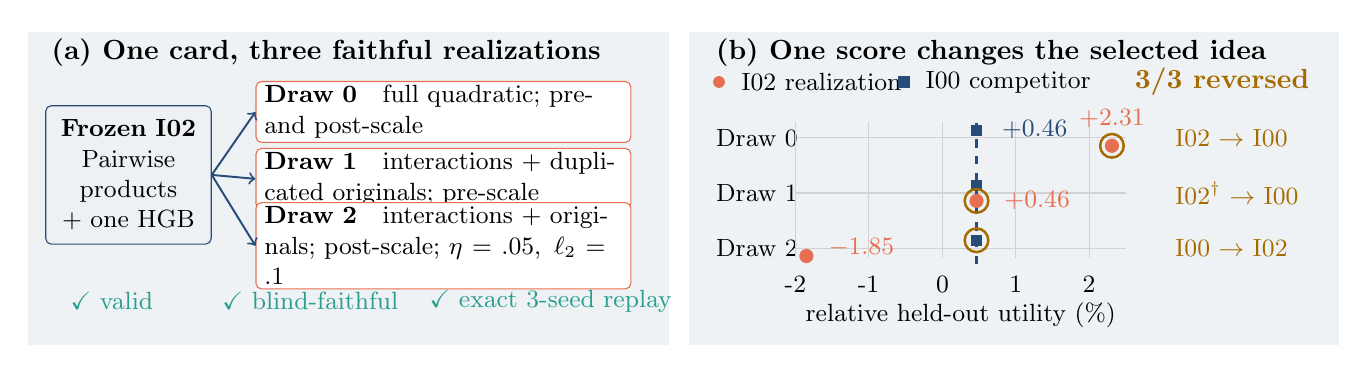
\begin{tikzpicture}[font=\small]
\path[use as bounding box] (0,-0.30) rectangle (16.65,3.75);
\fill[SoftGray] (0,-0.28) rectangle (8.15,3.70);
\fill[SoftGray] (8.40,-0.28) rectangle (16.65,3.70);
\node[anchor=west,font=\bfseries] at (0.18,3.43)
      {(a) One card, three faithful realizations};
\node[draw=IdeaBlue,fill=IdeaBlue!8,text width=1.75cm,align=center,
      rounded corners=2pt,inner sep=5pt] (card) at (1.28,1.88)
      {\textbf{Frozen I02}\\Pairwise products\\+ one HGB};
\node[draw=ImplCoral,fill=white,text width=4.55cm,align=left,
      rounded corners=2pt,inner xsep=3pt,inner ysep=1.5pt,
      minimum height=.56cm] (r0) at (5.28,2.68)
      {\textbf{Draw 0}\quad full quadratic; pre- and post-scale};
\node[draw=ImplCoral,fill=white,text width=4.55cm,align=left,
      rounded corners=2pt,inner xsep=3pt,inner ysep=1.5pt,
      minimum height=.56cm] (r1) at (5.28,1.83)
      {\textbf{Draw 1}\quad interactions + duplicated originals; pre-scale};
\node[draw=ImplCoral,fill=white,text width=4.55cm,align=left,
      rounded corners=2pt,inner xsep=3pt,inner ysep=1.5pt,
      minimum height=.56cm] (r2) at (5.28,0.98)
      {\textbf{Draw 2}\quad interactions + originals; post-scale;
       $\eta=.05,\ \ell_2=.1$};
\draw[->,IdeaBlue,line width=.7pt] (card.east) -- (r0.west);
\draw[->,IdeaBlue,line width=.7pt] (card.east) -- (r1.west);
\draw[->,IdeaBlue,line width=.7pt] (card.east) -- (r2.west);
\node[anchor=west,text=EvalTeal] at (0.42,0.28) {\(\checkmark\) valid};
\node[anchor=west,text=EvalTeal] at (2.35,0.28) {\(\checkmark\) blind-faithful};
\node[anchor=west,text=EvalTeal] at (4.98,0.28)
      {\(\checkmark\) exact 3-seed replay};

\node[anchor=west,font=\bfseries] at (8.62,3.43)
      {(b) One score changes the selected idea};
\fill[ImplCoral] (8.78,3.06) circle (.075);
\node[anchor=west] at (8.94,3.06) {I02 realization};
\fill[IdeaBlue] (11.05,2.985) rectangle +(0.15,0.15);
\node[anchor=west] at (11.28,3.06) {I00 competitor};
\node[anchor=east,text=AuditGold,font=\bfseries] at (16.40,3.06)
      {3/3 reversed};
\foreach \y/\lab in {2.35/Draw 0,1.65/Draw 1,0.95/Draw 2} {
  \draw[gray!35] (9.75,\y) -- (13.95,\y);
  \node[anchor=west] at (8.62,\y) {\lab};
}
\foreach \x/\lab in {9.75/{-2},10.68/{-1},11.62/{0},12.55/{1},13.48/{2}} {
  \draw[gray!35] (\x,0.82) -- (\x,2.55);
  \node[anchor=north] at (\x,0.72) {\lab};
}
\node[anchor=south] at (11.85,-0.18) {relative held-out utility (\%)};
\draw[IdeaBlue,dashed,line width=.8pt] (12.05,0.75) -- (12.05,2.55);
\foreach \y in {2.45,1.75,1.05} {
  \fill[IdeaBlue] (11.98,\y-.07) rectangle (12.12,\y+.07);
}
\node[anchor=west,text=IdeaBlue] at (12.25,2.45) {+0.46};
\fill[ImplCoral] (13.77,2.25) circle (.09);
\node[anchor=south,text=ImplCoral] at (13.77,2.36) {+2.31};
\fill[ImplCoral] (12.05,1.55) circle (.09);
\node[anchor=west,text=ImplCoral] at (12.28,1.55) {+0.46};
\fill[ImplCoral] (9.89,0.85) circle (.09);
\node[anchor=west,text=ImplCoral] at (10.05,0.96) {$-1.85$};
\draw[AuditGold,line width=.9pt] (13.77,2.25) circle (.15);
\draw[AuditGold,line width=.9pt] (12.05,1.55) circle (.15);
\draw[AuditGold,line width=.9pt] (12.05,1.05) circle (.15);
\node[anchor=west] at (14.45,2.35)
      {\textcolor{AuditGold}{I02 \(\rightarrow\) I00}};
\node[anchor=west] at (14.45,1.65)
      {\textcolor{AuditGold}{I02$^\dagger$ \(\rightarrow\) I00}};
\node[anchor=west] at (14.45,0.95)
      {\textcolor{AuditGold}{I00 \(\rightarrow\) I02}};
\end{tikzpicture}
\caption{Implementation lottery in one fresh-extension case (OpenML task 146822, Bounded), chosen after unblinding to illustrate the mechanism. Pooled inference is in Figure~\ref{fig:main}. The illustrated I02--I00 pair is semantically distinct. Three valid, blind-faithful I02 realizations yield $+2.31\%$, $+0.46\%$, and $-1.85\%$ relative utility, while each saved artifact replays exactly across three seeds. Against I00 ($+0.46\%$), every one-draw selection changes under the other-two mean. Omitted cards score zero. The dagger marks the frozen exact-tie rule.}
\label{fig:case}
\end{figure*}

\paragraph{A concrete implementation lottery.}
Figure~\ref{fig:case} makes the estimand tangible without adding a new inferential test. The three allowed realizations of the same interaction-feature card range from $+2.31\%$ to $-1.85\%$ relative held-out utility, and their prediction vectors disagree on as many as 4.76\% of examples. Against a competing card that remains at $+0.46\%$, all three one-shot choices are reversed by the other two implementations. Because every patch is executable and blind-faithful and its same-patch reruns agree exactly, ordinary implementation choices rather than failure, fidelity penalties, or rerun noise change the selected idea in this case.
A high-scoring artifact can remain valid even when its score provides limited evidence about the parent idea.

\subsection{The Lottery Persists Across Processes}

The implementation lottery appears in both setups. Phase~1 ICC is .661 for Bounded and .260 for Agentic, with 22.2\% and 66.7\% reversal. On seven fresh tasks the ordering flips. ICC is .588 versus .711, while reversal is 28.6\% versus 23.8\% (paired $p=1.00$). Pooled Agentic-minus-Bounded intervals include zero for ICC ($-.101$ [$-.337,.173$]) and reversal (+17.9\% [0.0\%, 38.5\%], $p=.1875$). These audits therefore do not identify a consistent reliability ordering between the two implementation processes. Reliability must be estimated for the process being evaluated.

\subsection{Execution Validity and Audit Trail}

All 312 assignments remain in ITT. Each setup has 147/156 valid assignments. The remaining nine are evaluation errors, with zero code-invalid patches. Fidelity is faithful or partial for 150/156 Bounded and 152/156 Agentic assignments. On the double-labeled subset, exact agreement is 47/49 and 43/49. The primary reviewer detects 50/52 and 51/52 constructed drifts and all 52/52 constructed invalids in each setup. The single missing response identifier noted above affects the completeness audit, not assignment inclusion.

Two outcome-blind repairs remain in the audit trail. A family classifier was corrected to use the mechanism field. Task~18 then has three rather than four families, but frozen cards were not regenerated. The registered ten generation attempts became a floor with a ceiling of 40 when some tasks produced too few distinct candidates. Tasks 3913 and 9952 required 14 and 13 attempts. Both repairs preceded hidden outcomes and left accepted cards unchanged.

\subsection{Portfolio Validity Is a Separate Gate}
\label{sec:portfolio-validity}

To test whether degenerate cards account for the reversals, we repeated the analysis after applying two outcome-blind card filters. A fresh-context OpenAI Codex instance from outside the DeepSeek pipeline reviewed only the 52 frozen Tabular cards and visible baselines after execution. A conservative rule flags any card that is not baseline-distinct, \mbox{single-mechanism}, representation- and policy-applicable, and idea-like, admitting 38/52 cards (73.1\%). Some flags reflect a review instruction stricter than the frozen protocol on fitted preprocessing and idea-versus-recipe boundaries. A construct-focused adjudication using the frozen policy therefore admits 43/52 (82.7\%). Substantive flags include monotone transforms that are effectively equivalent for histogram trees, one multi-mechanism umbrella, and one duplicate pair.

\begin{table}[b]
\centering
\small
\setlength{\tabcolsep}{5pt}
\caption{LOO winner reversal (\%) before and after outcome-blind card filtering. Every set retains all 13 tasks.}
\label{tab:portfolio-sensitivity}
\begin{tabular}{lrrr}
\toprule
Candidate set & Cards & Bounded & Agentic \\
\midrule
All frozen & 52 & 25.6 & 43.6 \\
Conservative rule & 38 & 43.6 & 35.9 \\
Construct rule & 43 & 33.3 & 38.5 \\
\bottomrule
\end{tabular}
\end{table}

Requiring all four cards in a task to pass is stricter than card-level filtering. Under the construct rule, five of seven excluded tasks contain only one flagged card. We therefore make card-level filtering the primary sensitivity. Keeping admitted cards and every task with at least two candidates retains all 13 tasks. Table~\ref{tab:portfolio-sensitivity} reports reversal of 33.3--43.6\%, with task-cluster intervals spanning 12.8--66.7\%. The unequal two-to-four cards per task preclude the registered balanced method-of-moments ICC. As a maximally conservative check requiring every card to pass, the conservative rule leaves four tasks (ICC .550/.250 and 50.0\% reversal in each setup). The construct rule leaves six (ICC .642/.443 and 33.3\% reversal in each), albeit with wide intervals.

We use the post-execution construct audit only for sensitivity analysis and leave both the cards and primary ITT sample unchanged. The all-13 estimates measure the reliability of the deployed candidate-card workflow. Clean mechanism-level promotion additionally requires the portfolio gate.

\subsection{The Lottery Persists in Materials}
\label{sec:materials}

Materials stress-tests cross-domain transfer and exposes a second failure mode. Its outcome-blind review passes band gap but flags baseline-equivalent, bundled, duplicate, or representation-dependent candidates in steels and phonons. Performance-only evaluation would miss this portfolio failure; prospective semantic admission is designed to catch it. We therefore treat all 72 assignments as exploratory and do not pool them with Tabular. Winner reversal is 33.3\% [0.0\%, 66.7\%] for Bounded and 55.6\% [0.0\%, 100.0\%] for Agentic. Frozen-card ICC is .290 [.000, .824] and .177 [.040, .777], with implementation shares of 71\% and 82\%. Same-artifact rerun variance is zero by construction because the evaluator is deterministic. Bounded validity is 29/36 (80.6\%), \mbox{below the registered .85 gate}, while Agentic validity is 34/36 (94.4\%). Intervals are wide because only three workflows are available. Even with rerun variation fixed at zero, however, implementation variation dominates and winner reversals remain.

\section{Related Work}

\paragraph{Automated research.} Automated research systems increasingly connect ideation, coding, execution, and selection. The AI Scientist, Dolphin, Agent Laboratory, Co-Scientist, ERA, execution-grounded research, specialist-agent recipe search, and closed-loop molecular workflows automate different parts of this loop \cite{lu2024aiscientist,yuan2025dolphin,schmidgall2025agentlab,gottweis2026coscientist,aygun2026era,si2026executiongrounded,ning2026specialists,ning2026molecular}. Related work studies end-to-end automation of AI research directly \cite{lu2026automation}. MLGym, MLRC-Bench, MLR-Bench, ResearchGym, and ResearchArena provide executable environments for research agents \cite{nathani2025mlgym,zhang2025mlrcbench,chen2025mlrbench,garikaparthi2026researchgym,zhang2026researcharena}. They test whether agents can complete research tasks or improve experimental artifacts. We study when this artifact-level feedback can be attributed to the idea that generated it.

\paragraph{Ideas and execution.} Research idea evaluation has scored written proposals for novelty and feasibility \cite{si2025ideas}. A closely related execution study assigns one completed project to each idea and shows that execution can change an idea's evaluation \cite{si2026gap}. We repeat fresh-session implementation attempts of the same idea to study the next measurement step. ResearchCodeBench, AutoExperiment, and AutoReproduce test whether agents can translate scientific intent into working code \cite{hua2025researchcodebench,kim2026autoexperiment,zhao2025autoreproduce}. Complementary analysis identifies implementation capability as a central bottleneck \cite{zhu2025implementation}. Our audit asks whether independently generated translations preserve the same idea-selection decision, with fidelity labeled separately.

\paragraph{Repeated trials.} Repeated-run evaluations expose agent inconsistency \cite{rabanser2026reliability,mehta2026disagree}. \mbox{Mustahsan et al.}\ quantify it with ICC \cite{mustahsan2025icc}. Pass@$k$ and self-consistency aggregate samples, while diverse query initialization searches trajectories \cite{chen2021codex,wang2023selfconsistency,murali2026divinit}. Rollout Cards preserves rollout-level evidence and its reporting rules \cite{masters2026rolloutcards}. Controlled second-pass studies decompose gains into re-solving, scaffold, and content effects \cite{ning2026revision}. Where these methods repeat a task or query, our audit fixes a semantic idea, samples independent translations, reruns saved artifacts, and tests winner stability. Best-of-$k$ remains complementary.

\paragraph{Measurement and experimental variance.} Machine learning experiments vary across seeds, splits, hyperparameters, models, and benchmarks \cite{henderson2018matters,bouthillier2021variance,agarwal2021precipice,wortsman2022modelsoups,dehghani2021benchmarklottery,liang2023helm,pineau2021reproducibility}. Those studies quantify uncertainty around specified pipelines. We repeat the translation of a semantic mechanism and ask whether legal realizations preserve its idea-level decision. Hyperparameters may be one open choice; fixing all choices yields a recipe, while tuning defines a richer implementation process. Construct-validity work separates a claimed concept from its measurement \cite{jacobs2021measurement,bean2025construct}, and we apply reliability tools to the idea-to-implementation mapping \cite{shrout1979icc,brennan2001generalizability}. Artifact-search systems such as FunSearch and AlphaEvolve make artifact-level claims \cite{romera2024funsearch,novikov2025alphaevolve}; idea reliability matters when their outputs credit a broader hypothesis or steer idea-level learning.

\section{Scope and Limitations}

The reported rates apply to this task pool, four candidates per task, three implementations, two same-provider implementation processes, and one evaluator. The all-13 estimates describe the deployed workflow. Because semantic review occurred after execution and depends on policy judgments, mechanism-level promotion should instead use prospective gating. ICC varies with candidate spread and our zero-bounding rule. LOO also depends on a frozen cross-card alignment because the provider did not expose sampling seeds. Accordingly, 25.6--43.6\% is conditional rather than an error rate for arbitrary projects. Fidelity labels were blinded and stress-tested but were not provided by humans, and ITT retains failure and drift. Materials was historically exposed and remains exploratory. We do not evaluate best-of-$N$ stability, end-to-end tree search, universal thresholds, or downstream audit gains. OpenML is comparatively constrained. Larger deep-learning workflows add choices in data, architecture, optimization, checkpoints, and systems, creating more routes from one realization to a different idea-level conclusion. Their reversal rates require measurement; attribution grows with workflow complexity.

\section{Implications for Automated Research}
\label{sec:implications}

\paragraph{Match evidence to the objective.} Best-of-$N$ search is appropriate for artifact delivery, whereas mechanism-level claims also require portfolio validity and reliability across implementations. Before a score prunes a branch, justifies transfer, enters research memory, or supports a mechanism-level claim, the candidate must denote a coherent intervention whose ranking survives another realization.

\paragraph{Supply evidence for promotion decisions.} Consequential checkpoints need not audit every candidate. The three-draw design triples executor assignments, while rerun calibration and fidelity review use only evaluator calls. A practical policy validates portfolios before implementation, requests additional implementations when candidates are close or implementation variation is high, and audits finalists before reusing their scores as evidence. Benchmark and leaderboard maintainers can adopt the schema to distinguish artifact scores from idea-level evidence. Large implementation variation calls for new implementations, rerun variation for a more stable evaluator, and low fidelity for tighter control.

\noindent The following schema is not a universal threshold.

\noindent\fbox{\begin{minipage}{0.92\columnwidth}\small
\textbf{Idea Reliability Audit checklist}\\[1pt]\hrule\vspace{2pt}
\textbf{Unit:} mechanism, invariants/open choices, portfolio gate.\\
\textbf{Process:} executor/model, budget, independence, repeats.\\
\textbf{Adherence:} blind validity/fidelity; failures retained in ITT.\\
\textbf{Noise:} byte-identical reruns and evaluator policy.\\
\textbf{Evidence:} idea ICC/uncertainty, LOO reversal, sensitivities.
\end{minipage}}

\paragraph{Build cumulative scientific knowledge.} Cumulative use requires evidence that a mechanism, not only one artifact, remains reliable across implementations. Idea reliability matters when mechanisms are compared, falsified, transferred, or recombined across machine learning, materials workflows, simulations, data-analysis plans, wet-lab procedures, and multi-agent research trajectories \cite{wang2023scientificdiscovery,gottweis2026coscientist}. It prevents a lucky realization or malformed candidate from steering the cumulative trajectory.

\section{Conclusion}

\emph{One run is not an idea.} Automated research systems often ask one realization-level score to do two jobs: deliver an artifact and decide which parent idea to retain, transfer, or remember. Best-of-$N$ search can serve the first objective, but the second requires evidence that survives another legitimate translation of the same mechanism. We call dependence on the sampled translation the \emph{implementation lottery}; \emph{idea reliability} is the stability of idea-level evidence across such translations.

The \emph{Idea Reliability Audit} holds mechanism-level cards fixed, translates each card in three fresh sessions, uses outcome-blind fidelity labels, retains failure and drift under ITT, and reruns saved artifacts unchanged. Idea ICC measures how much within-task variation separates ideas, while LOO reversal asks whether a one-draw winner survives the other two implementations. Across 312 assignments on 13 tabular tasks, implementation choice accounts for 33\% and 45\% of within-task ITT variance, more than fivefold and tenfold the same-artifact rerun variance. One-draw winners reverse in 25.6\% and 43.6\% of sampled LOO decisions. The lottery persists in Bounded and Agentic, although their ordering reverses in the fresh extension. Outcome-blind card filtering retains all 13 tasks and leaves reversal at 33.3--43.6\%, so flagged degeneracies do not explain the result. An exploratory Materials diagnostic shows the same directional pattern under deterministic evaluation and exposes portfolio validity as a separate gate.

Together, these findings distinguish average-realization idea quality from best-of-$N$ artifact utility. Search can optimize the delivered artifact; mechanism-level branching, transfer, and research memory additionally require evidence that survives multiple implementations. The measured rates vary by setting, but the attribution problem is structural whenever a realization updates beliefs about an idea. Search delivers artifacts; the audit supports cumulative science.

\clearpage
\bibliography{aaai2027}

\end{document}
